\documentclass [dvipsnames] {article}


\title {Projekt Równania Różniczkowe i Różnicowe Dokumentacja}
\date {24.01.2020}
\author {Kamil Burkiewicz}


	% równania bez znaczników
\usepackage {amsmath}

	% polskie znaki
\usepackage{polski}
\usepackage[utf8]{inputenc}

	% jakieś fonty + liczby rzeczywiste
\usepackage{amsfonts}
	% obrazki
\usepackage{graphicx}
\graphicspath{ {./} }


\begin {document}

	\pagenumbering {gobble}
	\maketitle
	\newpage

	\tableofcontents
	\newpage
	\pagenumbering {arabic}

		% section 1
	\section {Sformułowanie Wariacyjne}


	Przedstawiony został następujący problem:\\
	Przybliżenie rozwiązania równania różniczkowego metodą elementów skończonych
	\begin {equation*}
		-(a(x)u'(x))' + b(x)u'(x) + c(x)u(x) = f(x)
	\end {equation*}

	\begin {equation*}
		-\frac{d^2u}{d x^2}  (x) - u(x) = 0
	\end {equation*}	
	
	\begin {equation*}
		u(0) = 0
	\end {equation*}	
	
	\begin {equation*}
		\frac{du}{dx} (2) - u(2) = 0
	\end {equation*}	

	\begin {equation*}
		[0,2] \ni x \mapsto u(x) \in \mathbb{R}
	\end {equation*}
	
	Rozwiązanie:

	\begin {equation*}
		-u''(x) - u(x) = 0
	\end {equation*}
	
	\begin {center}
		Mnożymy obie strony równania przez funkcję próbną $v \in V = \{e_0, ..., e_n \}$
	\end {center}
	\begin {equation*}
		-u'' \cdot v - u \cdot v = 0,
	\end {equation*}
	
	\begin {equation}	%equaiton 1
		\int_{0}^{2} -u'' \cdot v dx - \int_{0}^{2}u \cdot vdx = 0
	\end {equation}
	\begin {center}
		Zajmujemy się teraz pierwszą całką:
	\end {center}
	\begin {equation*}
		\int_{0}^{2} -u'' \cdot vdx = 
		\begin {vmatrix}
			v     &     v' \\
			-u''  &    -u'
		\end {vmatrix}
		= [-u' \cdot v]_{0}^{2} + \int_{0}^{2} u' \cdot v'dx =
	\end {equation*}
	\begin {equation*}
		= -u'(2) \cdot v(2) + u'(0) \cdot v(0) + \int_{0}^{2} u' \cdot v'dx =
		-u(2) \cdot v(2) + \int_{0}^{2} u' \cdot v'dx 
	\end {equation*}
	\begin {center}
		Wstawiamy otrzymany wynik do równania (1) i otrzymujemy:
	\end {center}	
	\begin {equation}	% equation 2
		-u(2) \cdot v(2) + \int_{0}^{2} u' \cdot v'dx - \int_{0}^{2}u \cdot vdx = 0
	\end {equation}
	
	\begin {center}
		Przyjmujemy, że rozwiązanie jest kombinacją liniową funkcji bazowych, czyli
		 $$u = \sum_{i=0}^{i=n} c_i \cdot e_i $$ dla pewnych stałych $c_i, i = 0,...,n$ \\
		Wstawiamy przewidywaną formę u do równania (2) oraz wstawiamy za funkcje próbną $e_j$, dla $j = 0,...,n$.
		Otrzymujemy n + 1 równań postaci
	\end {center}
	$$-\sum_{i = 0}^{n} c_i \cdot e_i(2) \cdot e_j(2) + \int_{0}^{2} (\sum_{i = 0}^{n} c_i \cdot e_i)' \cdot e_j' dx - \int_{0}^{2}\sum_{i = 0}^{n}c_i \cdot e_i \cdot e_j dx = 0 $$
	\begin {center}
		Z liniowości całki, pochodnej oraz operatora sumowania:
	\end {center}
	$$ \sum_{i = 0}^{n} c_i \cdot (-e_j(2) \cdot e_i(2)) + \sum_{i = 0}^{n} c_i \int_{0}^{2} e_i' \cdot e_j' dx - \sum_{i = 0}^{n} c_i \int_{0}^{2} e_i \cdot e_j dx = 0 $$

	$$ \sum_{i = 0}^{n} c_i \cdot (-e_j(2) \cdot e_i(2) + \int_{0}^{2} (e_i' \cdot e_j' - e_i \cdot e_j) dx) = 0 $$
	
	\begin {center}
		Przyjmijmy teraz:
	$$ a_{ij} := -e_i(2) \cdot e_j(2) + \int_{0}^{2} (e_i' \cdot e_j' - e_i \cdot e_j) dx $$
	Co po podstawieniu daje:
	$$ \sum_{i = 0}^{n} c_i \cdot a_{ij} = 0 $$
		n + 1 równań o n+1 niewiadomych $c_i$ można zapisać w postaci układu jednorodnego równań liniowych:
	\end {center}
	\begin {equation}	%equation 3
		A \cdot C = 0
	\end {equation}
	\begin {center}
			Dodatkowo
	$$ a_{ji}  = -e_j(2) \cdot e_i(2) + \int_{0}^{2} (e_j' \cdot e_i' - e_j \cdot e_i) dx = a_{ij} $$
	czyli w tym przypadku macierz A będzie symetryczna.
	\end {center}
	\begin {equation*}
		A = [a_{ij}]_{n+1 \times n+1}, C = [c_i]_{n+1 \times 1}, 0 = [0]_{n+1 \times 1}
	\end {equation*}
	\begin {center}
		Należy znaleźć macierz $A^{-1}$ i pomnożyć przez nią lewostronnie równianie (3). \\
		Możemy zauważyć, że jeżeli isteniej macierz $A^{-1}$ to po pomnożeniu dostaniemy rozwiązanie zerowe. \\
		Odpowiednie obliczenia numeryczne zostaną jednak wykonane.
	\end {center}
	
		% section 2
	\newpage
	\section {Wyniki}

	Ze względu na zerowy warunek Dirichleta w punkcie 0 pominąłem funkcję bazową $e_0$.
	Do numerycznego obliczania całek używam kwadratury Gaussa-Legendra. Jest również procedura wbudowana w program MATLAB,
	która jest zapisana w kodzie, lecz wykomentowana i dostępna jeśli zaszłaby potrzeba otrzymania dokładniejszych wyników.
	Obliczam również współczynniki i węzły dla kwadratury Gaussa-Legendra na samym początku programu używając 3ciego wielomianu Legendra.
	Numer wielomianu Legendra jest do ustalenia, jako stała na początku programu. \\ \\

	\begin {flushleft}
	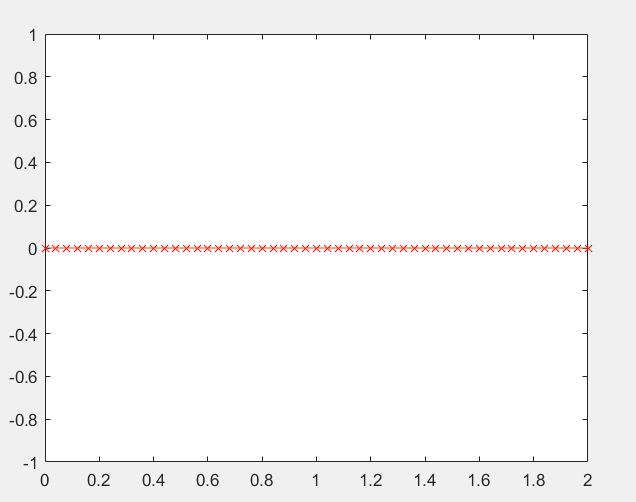
\includegraphics{DiffEqSolution1}	
	\end{flushleft}
	\begin {center}
		Rozwiązanie dla podziału na 50 podprzedziałów:
	\end {center}
	
	\newpage
	
	Jako, że program został napisany stosując wszelkie możliwe uogólnienia przedstawiam również rozwiązanie równania 
	$$ u'' + u = sin(x)$$
	dla analogicznych warunków brzegowych na przedziale $[0, \frac {\pi}{2}]$
	
	\begin{figure}[h!]
	\centering
	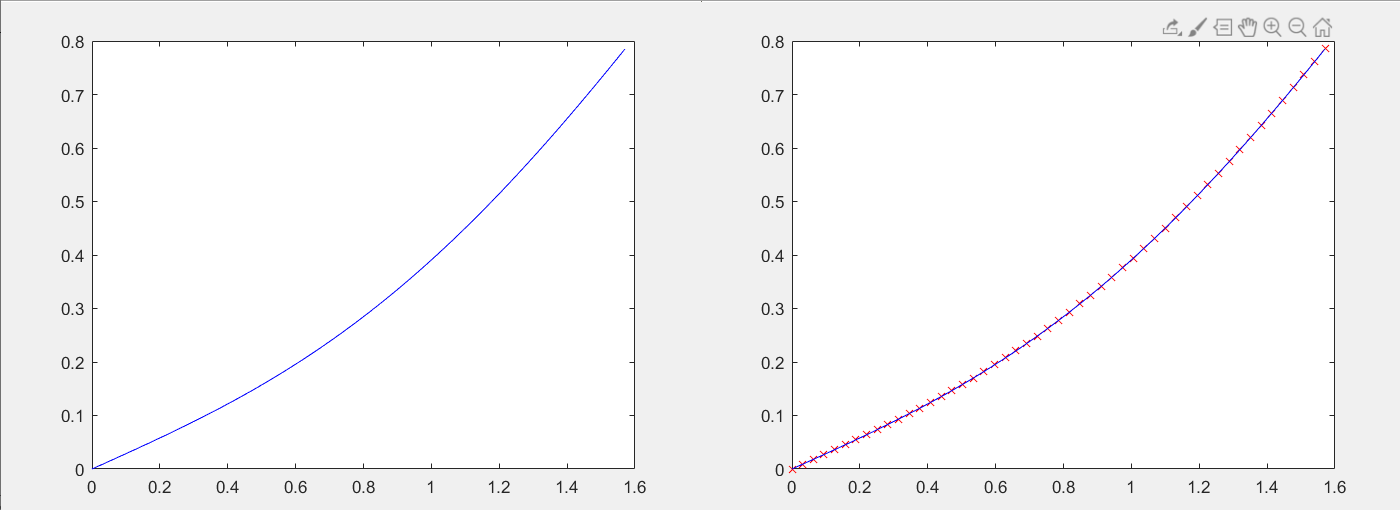
\includegraphics[scale = 0.5]{DiffEqSolutionExample}
	\caption{Lewy: rozwiązanie dokładne;  Prawy: MES}
	\label{fig:method}
	\end{figure}
	

\end {document}